\documentclass[a4paper,zihao=5,UTF8]{ctexart}
\usepackage[top=2.3cm,bottom=2cm,left=1.7cm,right=1.7cm]{geometry} 
\usepackage{amsmath, amssymb}
\usepackage{color}
\usepackage{hyperref} 
\usepackage{pythonhighlight}
\usepackage{listings}
\usepackage{mathrsfs} 
\usepackage{booktabs}
\usepackage{amsthm}
\usepackage{longtable} 
\usepackage{graphicx}
\usepackage{subfigure}
\usepackage{caption}
\usepackage{fontspec}
\usepackage{titlesec}
\usepackage{fancyhdr}
\usepackage{latexsym}
\usepackage{subfigure}
\usepackage{braket}
\usepackage{cite}
\usepackage[version=4]{mhchem}

\CTEXsetup[format={\Large\bfseries}]{section}
\def\d{\mathrm{d}}
\def\e{\mathrm{e}}
\def\i{\mathrm{i}}
\def\dps{\displaystyle}
\newcommand{\mr}[1]{\mathrm{#1}}
\newcommand{\mb}[1]{\mathbf{#1}}
\newcommand{\dv}[2]{\frac{\d{#1}}{\d{#2}}}
\newcommand{\pdv}[2]{\frac{\partial{#1}}{\partial{#2}}}
\def\degree{$^{\circ}$}
\def\celsius{$^{\circ}\mr{C}$}
\title{\textbf{偏微分方程数值解上机作业1}}
\author{王崇斌\;2201110455}
\makeatletter
\makeatother
\begin{document}
	\pagestyle{fancy}
	\pagestyle{fancy}
    \lhead{偏微分方程数值解}
	\chead{}
	\rhead{\today}
	\maketitle
    \thispagestyle{fancy}

	\section{单位圆盘上的Poisson方程}

	\begin{equation}
		\left\{
			\begin{aligned}
				&-\Delta u = 1, \quad (x, y) \in B\\
				&u(x, y) = 0, \quad (x, y) \in \partial B\\
				&B = \{(x, y), x^2 + y^2 < 1\}
			\end{aligned}
		\right.
	\end{equation}

	\subsection{极坐标中的差分格式}
	利用极坐标中Laplace算子的表达式$\dps\Delta = \frac{1}{r}\pdv{}{r}\left(r\pdv{}{r}\right) + \frac{1}{r^2}\pdv{^2}{\theta^2}$
	, 可以将上述直角坐标中的Poisson方程改写为如下形式, 额外补充了圆心处的有界性条件:
	\begin{equation}
		\left\{
			\begin{aligned}
				&-\frac{1}{r}\pdv{}{r}\left(r\pdv{u}{r}\right) - \frac{1}{r^2}\pdv{^2u}{\theta^2} = 1, \quad (r, \theta) \in (0, 1)\times[0, 2\pi)\\
				&u(1, \theta) = 1, \quad \theta \in [0, 2\pi)\\
				&\lim_{r \to 0^+} \pdv{u}{r} = 0, \quad \theta \in [0, 2\pi)
			\end{aligned}
		\right.
	\end{equation}
	可以看到方程与边界条件都具有$\theta$方向的平移对称性(或者说是直角坐标中的旋转对称性), 因此
	可以推断方程的解只是$r$的函数, 上述方程进一步可以改写为一个二阶常微分方程的边值问题:
	\begin{equation}
		\left\{
			\begin{aligned}
				&-\frac{1}{r}\dv{}{r}\left(r\dv{u}{r}\right) = 1, \quad r\in(0, 1)\\
				&u(1) = 0\\
				&\left.\dv{u}{r}\right|_{r = 0+} = 0
			\end{aligned}
		\right.
		\label{poisson r ode}
	\end{equation}
	为了利用半整点法构造$r=0$处的边界条件, 需要仔细构造网格, 令$\Delta r = \frac{1}{N-0.5},\,r_j = \frac{j - 0.5}{N - 0.5},\, j = 0, 1,\cdots, N$, 在这样的网格下$r_{0.5} = \frac{r_0 + r_1}{2}$
	为数轴上$r=0$的点, 采用中心差分逼近内点处的导数, 在$r_N$处采用Dirichlet边界条件, 
	在$r = 0$处采用半整点法构造边界条件, 
	得到如下差分格式:
	\begin{equation}
		\left\{
			\begin{aligned}
				& -\frac{1}{\Delta r^2\cdot r_j}\left[r_{j + 0.5}\left(u_{j+1} - u_j\right) - r_{j - 0.5}\left(u_j - u_{j - 1}\right)\right] = 1, \quad j = 1,\cdots, N-1\\
				&u_{N} = 0\\
				&\frac{u_1 - u_0}{\Delta r} = 0
			\end{aligned}
		\right.
	\end{equation}
	利用边界条件, 上述差分方程可以转化为N-1个未知数的三对角线性方程组:
	\begin{equation}
		\begin{bmatrix}
			\frac{r_{1.5}}{r_1} & -\frac{r_{1.5}}{r_1} & & & \\
			 & \ddots & & & \\
			 & -\frac{r_{j - 0.5}}{r_j} & 2 & -\frac{r_{j + 0.5}}{r_j} & \\
			 & & & \ddots & \\
			 & & & -\frac{r_{N - 1.5}}{r_{N-1}} & 2
		\end{bmatrix}
		\cdot
		\begin{bmatrix}
			u_1 \\
			\vdots\\
			u_j\\
			\vdots\\
			u_{N-1}
		\end{bmatrix}
		=
		\begin{bmatrix}
			\Delta r^2\\
			\vdots \\
			\Delta r^2 \\
			\vdots \\
			\Delta r^2
		\end{bmatrix}
	\end{equation}
	求解这个线性方程组, 即可得到Poisson方程的解.
	
	\subsection{精确解与数值解的比较}
	将方程[\ref{poisson r ode}]两边同时乘$r$后积分, 再除以$r$积分, 可以得到不考虑边值时的方程的通解:
	\begin{equation}
		u = -\frac{r^2}{4} + C_1\ln r + C_2
	\end{equation}
	带入[\ref{poisson r ode}]的边值条件后可以得到方程的精确解:
	\begin{equation}
		u = -\frac{r^2}{4} + \frac{1}{4} = -\frac{x^2 + y^2}{4} + \frac{1}{4}
	\end{equation}
	数值计算时采用LU分解求解线性方程组, 使用了之前学习某课程时编写的数值线性代数代码
	(My\_Matrix.cpp, My\_Matrix.h), 由于矩阵很小因此没有对三对角求解做特殊优化. 
	计算、编译、绘图程序分别参见 1\_poisson\_solver.cpp, compile1.bat, 1\_poisson\_plot.py
	. 将$N_r = 8, 16$的数值结果与精确结果绘图比较, 参见图(\ref{1 poisson Nr 8}), (\ref{1 poisson Nr 16}), 精度竟然会如此之高.
	\begin{figure}[htbp]
		\centering
		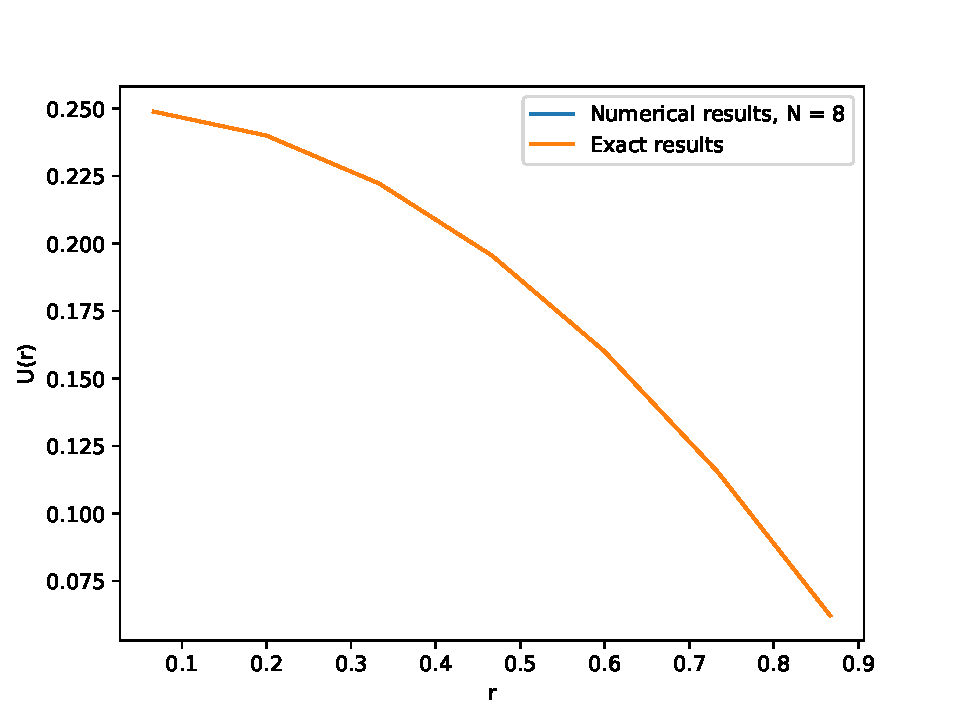
\includegraphics[scale=0.7]{1_poisson_Nr_8.pdf}
		\caption{$N_r$ = 8时数值解与精确解的结果比较}
		\label{1 poisson Nr 8}
	\end{figure}
	\begin{figure}[htbp]
		\centering
		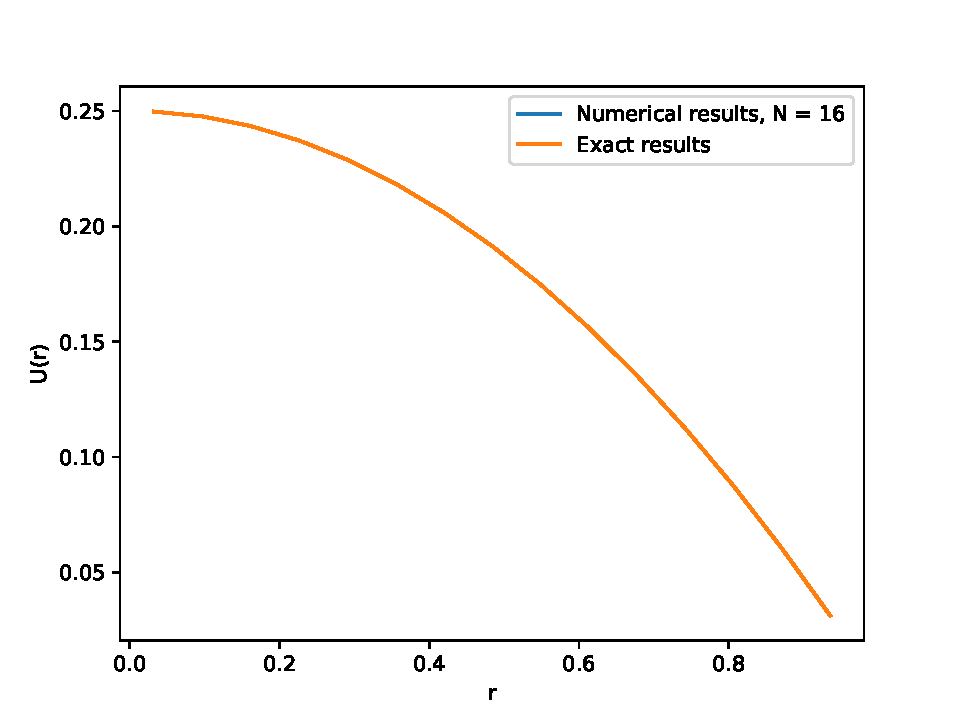
\includegraphics[scale=0.7]{1_poisson_Nr_16.pdf}
		\caption{$N_r$ = 16时数值解与精确解的结果比较}
		\label{1 poisson Nr 16}
	\end{figure}

	\section{扩散方程的初边值问题}
	\begin{equation}
		\left\{
			\begin{aligned}
				&\pdv{u}{t} = \pdv{^2U}{x^2},\quad x\in(0, 1),\,t > 0\\
				&u(x, 0) = \frac{x^2}{2}, \quad x\in [0, 1]\\
				&u(0, t) = 0, \, \pdv{u}{x}(1, t) = 1,\quad t > 0
			\end{aligned}
		\right.
	\end{equation}

	\subsection{显格式的后验误差估计}
	这一题由于给定了$\Delta x$, 使用半整点法无法解决, 被迫尝试使用影子节点法构造边界条件, 
	在[0, 1]之间按照题目给定间距$\Delta x$插入N个点, 使得$x_0 = 0, \,x_N = 1$, 在$x_N$右侧\
	$\Delta x$处插入影子节点$x_{N+1}$, 差分方程可以写为:
	\begin{equation}
		\left\{
			\begin{aligned}
				&\frac{u_{j}^{m+1} - u_{j}^{m}}{\Delta t} = \frac{1}{\Delta x^2}\left(u_{j+1}^{m} - 2u_{j}^{m} + u_{j - 1}^{m}\right), \quad j = 1, 2, \cdots, N\\
				&u_j^{0} = \frac{x_j^2}{2},\quad j = 0, 1, \cdots, N\\
				&u_{0}^{m} = 0,\quad m > 0\\
				&\frac{u_{N+1}^m - u_{N-1}^m}{2\Delta x} = 1, \quad m > 0
			\end{aligned}
		\right.
	\end{equation}
	将边界条件带入可以得到如下的显式递推关系, 其中网格比$\dps\mu = \frac{\Delta t}{\Delta x^2}$:
	\begin{equation}
		\left\{
			\begin{aligned}
				&u_{j}^{m+1} = \mu(u_{j+1}^m + u_{j-1}^m) + (1-2\mu)u_{j}^m, \quad j = 1, 2, \cdots, N-1\\
				&u_{N-1}^{m+1} = 2\mu(\Delta x + u_{N-1}^{m}) + (1 - 2\mu)u_{N}^{m}
			\end{aligned}
		\right.
	\end{equation}
	编写程序2\_diffusion\_explicit.cpp计算不同网格参数时$T=1$的解
	(编译使用命令g++ 2\_diffusion\_explicit.cpp -o 2\_diffusion\_explicit.exe -O3), 
	使用程序2\_1\_error.py计算收敛阶, 计算时使用公式:
	\begin{equation}
		\ln ||U_h - U_{h/2}|| \approx \ln [(1 - 2^{-\alpha})C] - \alpha \ln h^{-1}
	\end{equation}
	可以得到如图(\ref{2-1-error})所示的收敛阶示意图, 
	\begin{figure}[htbp]
		\centering
		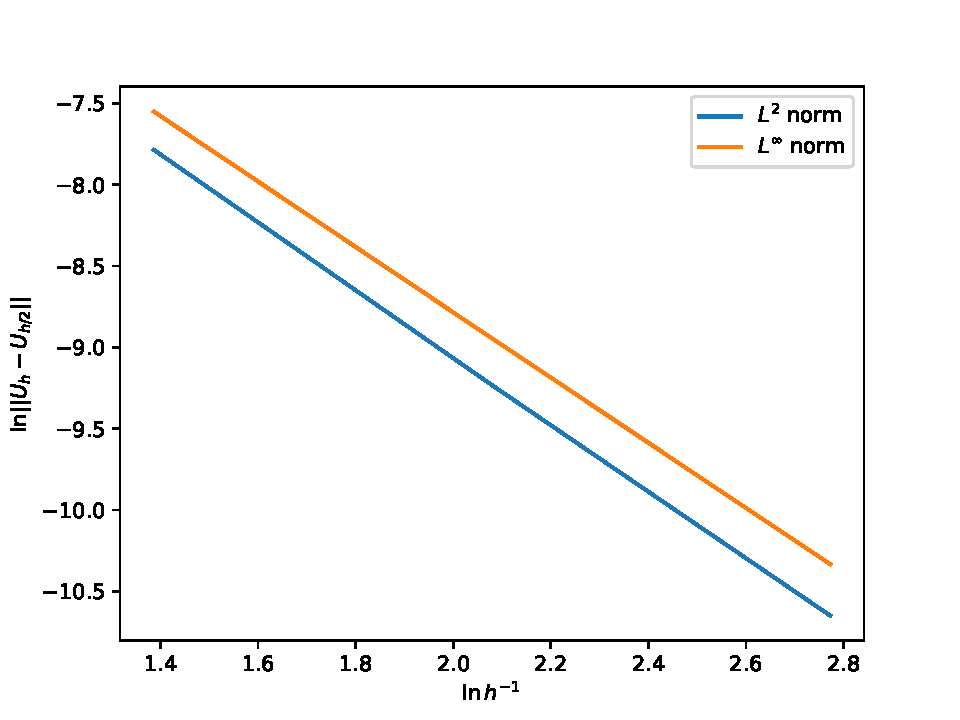
\includegraphics[scale=0.7]{2_1_error.pdf}
		\caption{扩散方程显式格式后验误差分析示意图}
		\label{2-1-error}
	\end{figure}
	选取后两个数据点计算收敛阶, 可以得到两种范数下的收敛阶为$\alpha_{\mr{L}^{2}} = 2.044,\,\alpha_{\mr{L}^{\infty}} = 2.003$

	\subsection{Crank-Nicolson格式}
	同样使用影子节点法处理右端边界条件, 将Crank-Nicolson格式应用于此问题, 可以给出如下差分格式:
	\begin{equation}
		\left\{
			\begin{aligned}
				&\frac{u_j^{m+1} - u_j^m}{\Delta t} = \frac{1}{2}\left(\frac{u_{j+1}^m - 2u_j^{m} + u_{j-1}^{m}}{\Delta x^2} + \frac{u_{j+1}^{m+1} - 2u_{j}^{m+1} + u_{j-1}^{m+1}}{\Delta x^2}\right), \quad j = 1, 2,\cdots, N\\
				&u_0^m = 0,\quad m > 0\\
				&\frac{u_{N+1}^m - u_{N-1}^{m}}{2\Delta x} = 1, \quad m > 0
			\end{aligned}
		\right.
	\end{equation}
	上经过一些运算, 上式所示的单步演化可以转化为一个三对角线性方程组的求解, 其中已经带入了$x=0, x=1$
	处边界条件:
	\begin{equation}
		\begin{bmatrix}
			\mu + 1 & -\frac{\mu}{2} & & & \\
			 & \ddots & & & \\
			 & -\frac{\mu}{2} & \mu + 1 & -\frac{\mu}{2} & \\
			 & & & \ddots & \\
			 & & & -\mu & \mu + 1
		\end{bmatrix}
		\cdot
		\begin{bmatrix}
			u_1^{m+1} \\
			\vdots\\
			u_j^{m+1}\\
			\vdots\\
			u_{N}^{m+1}
		\end{bmatrix}
		=
		\begin{bmatrix}
			\frac{\mu}{2}u_2^m + (1-\mu)u_1^m\\
			\vdots \\
			\frac{\mu}{2}u_{j+1}^m + (1-\mu)u_j^m + \frac{\mu}{2}u_{j-1}^m\\
			\vdots \\
			2\mu\Delta x + \mu u_{N-1}^m + (1-\mu)u_{N}^m
		\end{bmatrix}
	\end{equation}
	编写程序2\_diffusion\_CN.cpp计算不同时刻的$u$(编译使用compile2.bat),
	线性方程组的求解采用LU分解方法, 使用程序2\_2\_CN\_plot.py绘制图像. 将以$u(x, 0) = \frac{x^2}{2}$
	为初值的解作图, 参见图(\ref{2-2-CN-1}). 
	\begin{figure}[htbp]
		\centering 
		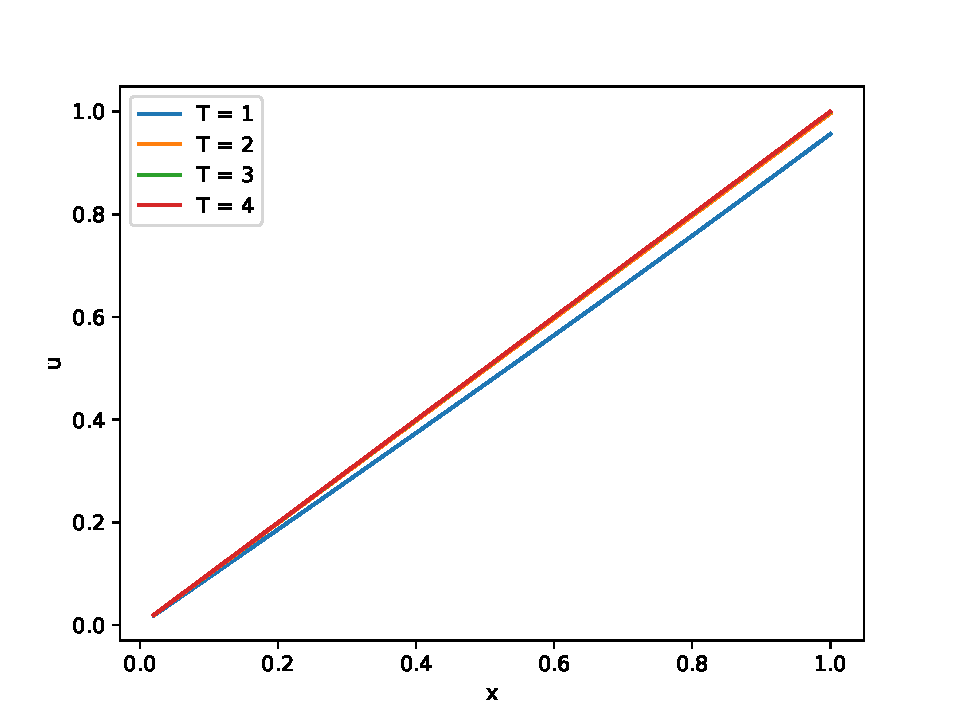
\includegraphics[scale=0.7]{2_2_CN_1.pdf}
		\caption{Crank-Nicolson格式求解以$u(x, 0) = \frac{x^2}{2}$为初值的扩散方程的解}
		\label{2-2-CN-1}
	\end{figure} 
	在程序2\_diffusion\_CN.cpp中将初始条件替换为$u(x, 0) = x^2 - x$, 重复编译计算并绘图, 参见图(\ref{2-2-CN-2}). 
	\begin{figure}[htbp]
		\centering 
		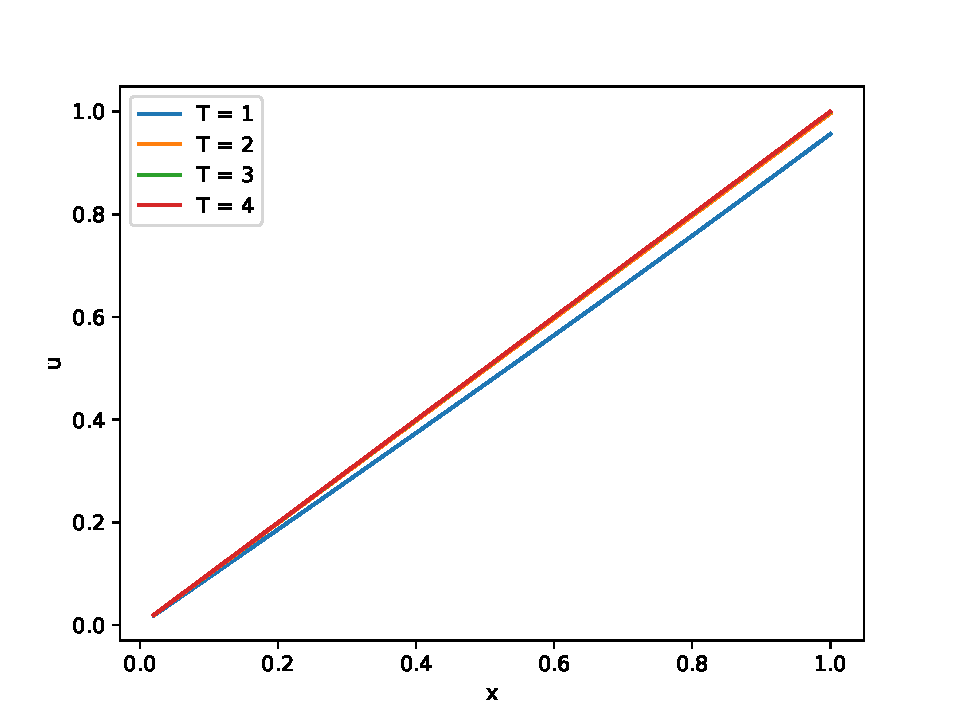
\includegraphics[scale=0.7]{2_2_CN_1.pdf}
		\caption{Crank-Nicolson格式求解以$u(x, 0) = x^2 - x$为初值的扩散方程的解}
		\label{2-2-CN-2}
	\end{figure} 
	观察这两种不同初值条件下扩散方程解的行为, 发现两者在足够长的时间后趋于同样的解$u(x) = x$, 这
	说明在适当的边界条件下(比如一端流入一端流出, 总不能是两端都流入), 扩散方程存在
	稳态解$u(x, +\infty)$, 如果稳态解存在, 对应的就是同样边界条件下Laplace(Poisson)方程的解.

	\section{一阶波方程的初边值问题}
	\begin{equation}
		\left\{
			\begin{aligned}
				&\pdv{u}{t} + \pdv{u}{x} = 0,\quad x\in(0, 5),\,t > 0\\
				&u(x, 0) = \e^{-5(x - 1)^2}, \quad x\in [0, 5]\\
				&u(-1, t) = 0, \quad t > 0
			\end{aligned}	
		\right.
	\end{equation}
	\subsection{一阶upwind方法的后验误差估计}
	由于不涉及复杂边界条件的处理, 可以采用[-1, 5]之间间距为$\Delta x$的均匀网格, 由于
	流速大于0, 迎风格式可以写为:
	\begin{equation}
		\left\{
			\begin{aligned}
				&u_j^{m+1} = (1 - \nu)u_j^m + \nu u_{j-1}^m, \quad m > 0,\,j = 1, 2, \cdots, N\\
				&u_0^m = 0,\quad m > 0\\
				&u^0_j = \e^{-5(x_j - 1)^2}, \quad j = 0, 1, \cdots, N
			\end{aligned}
		\right.
	\end{equation}
	其中网格比选为$\nu = 0.5$, $\Delta t = \nu \cdot \Delta x$, 
	编写程序3\_1\_upwind.cpp计算不同$\Delta x$时的数值结果, 使用程序3\_1\_error.py(
	后验误差估计的逻辑与第二题类似), 可以得到如图(\ref{3-1-upwind})所示的收敛阶示意图, 
	\begin{figure}[htbp]
		\centering
		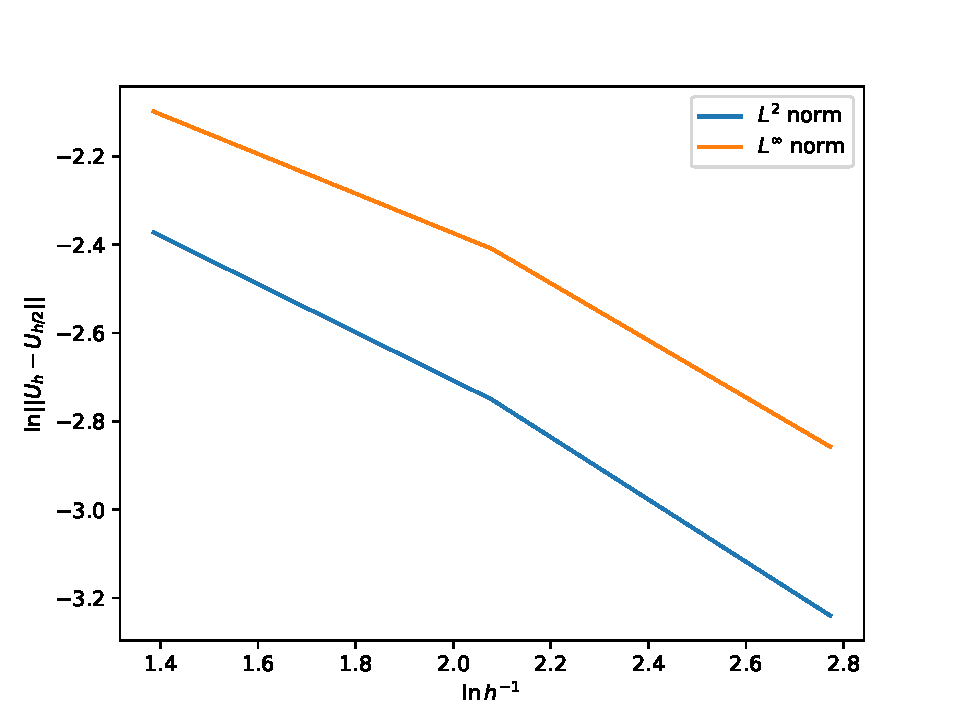
\includegraphics[scale=0.7]{3_1_error.pdf}
		\caption{upwind格式的后验误差分析示意图}
		\label{3-1-upwind}
	\end{figure}
	可以根据后两个数据点计算出两种范数下的收敛阶为$\alpha_{\mr{L}^{2}} = 0.705,\,\alpha_{\mr{L}^{\infty}} = 0.646$, 能够看出收敛阶并不是非常接近理论值1, 观察示意图, 可以看出收敛阶还没有
	对$\Delta x$收敛, 这可能是因为upwind格式精度较低导致收敛阶收敛变慢, 
	预计进一步减小$\Delta x$可能会得到更准确的收敛阶. 令$\Delta x = \frac{1}{64}, \frac{1}{128}, \frac{1}{256}$, 重新绘制收敛阶的示意图(\ref{3-1-upwind-new}), 
	\begin{figure}[htbp]
		\centering
		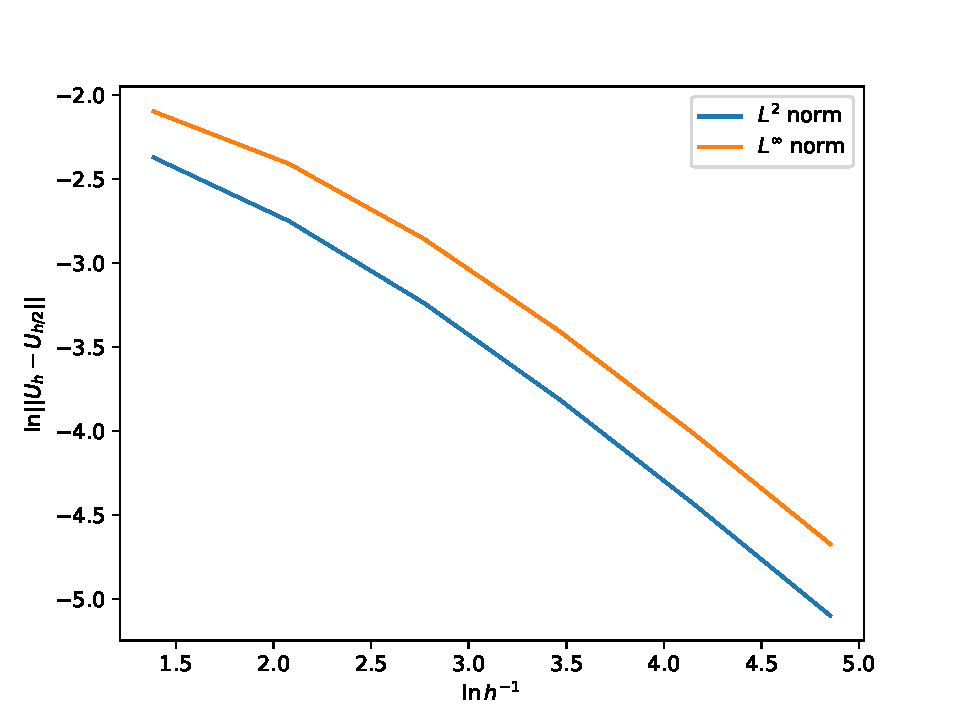
\includegraphics[scale=0.7]{3_1_error_new.pdf}
		\caption{upwind格式的后验误差分析示意图}
		\label{3-1-upwind-new}
	\end{figure}
	此时计算出两种范数下的收敛阶为$\alpha_{\mr{L}^{2}} = 0.950,\,\alpha_{\mr{L}^{\infty}} = 0.940$
	, 这就体现出了理论上的收敛阶.

	\subsection{不同网格比时upwind格式的行为}
	继续使用上一题的程序, 修改其中$\nu = 0.5, 1, 2$, 维持$\Delta x = \frac{1}{32}$, 将得到的
	解绘制在图(\ref{3-2-upwind-compare})中, 
	\begin{figure}[htbp]
		\centering
		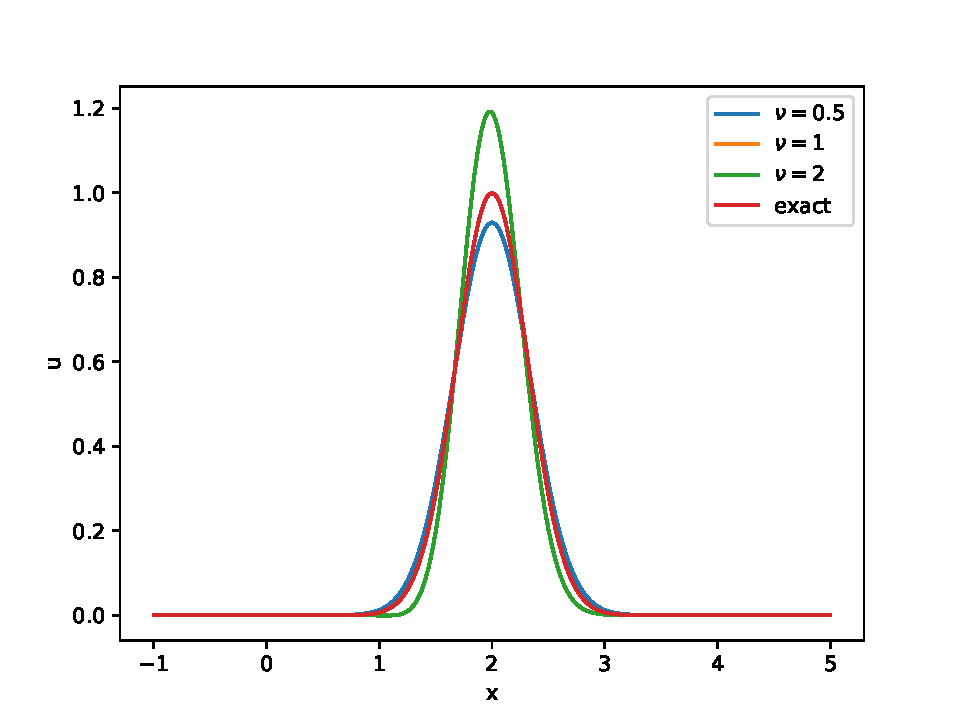
\includegraphics[scale=0.7]{3_2_upwind_compare.pdf}
		\caption{使用不同网格比$\nu = 0.5, 1, 2$时波方程的解}
		\label{3-2-upwind-compare}
	\end{figure}
	观察网格比$\mu$不同的解, 可以观察到$\nu = 1$时的解与精确解严格一致, 而$\nu = 0.5$数值解有
	明显的耗散现象(波峰降低). $\nu = 2$的解不满足CFL条件, 可以看出高斯波形的边缘开始出现小于0的
	部分(震荡), 而在波峰处开始出现增长(发散), 这表明不满足CFL条件的数值解不能正确描述方程的演化.
	\par 
	利用Von-Neumann分析, 能够得到增长因子和相位的表达式:
	\begin{equation}
		\left\{
			\begin{aligned}
				& |\lambda_k|^2 = 1 - 4\nu(1-\nu)\sin^2\left(\frac{k\Delta x}{2}\right)\\
				&\arg\lambda_k = -\arctan\left[\frac{\nu\sin k\Delta x}{(1-\nu) + \nu\cos k\Delta x}\right]
			\end{aligned}
		\right.
	\end{equation}
	可以看到当$\nu = 1$时, 对于任意波数$k$的Fourier波形, 均不会产生振幅和相位的误差, 因此从
	理论上讲此种情形的数值解是精确的.

	\subsection{Lax-Wendroff格式}
	如果利用Lax-Wendroff格式, 需要在右边边界上补充一个边界条件, 为了更好观察到高斯波形的传播
	(也是为了便于数值计算), 我打算采用无反射边界条件, 补充影子节点$u_{N+1}^m = u_N^m$, 
	可以构造如下的差分格式:
	\begin{equation}
		\left\{
			\begin{aligned}
				&u_j^{m+1} = -0.5 \nu(1-\nu)u_{j+1}^m + (1 - \nu^2)u_j^{m} + 0.5 \nu(1+\nu)u_{j-1}^m, \quad j = 1, 2, \cdots, N\\
				&u_{N}^m = u_{N+1}^m
			\end{aligned}
		\right.
	\end{equation}
	将边界条件带入可以得到显式递推关系:
	\begin{equation}
		\left\{
			\begin{aligned}
				& u_0^m = 0\\
				& u_j^{m+1} = -0.5 \nu(1-\nu)u_{j+1}^m + (1 - \nu^2)u_j^{m} + 0.5 \nu(1+\nu)u_{j-1}^m, \quad j = 1, 2, \cdots, N - 1\\
				& u_{N}^{m+1} = (-0.5 \nu + 1 - 0.5\nu^2)u_{N}^m + 0.5\nu(1+\nu)u_{N-1}^m
			\end{aligned}
		\right.
	\end{equation}
	在计算中采用$\nu = 0.5, \Delta x = 1/100$, 编写程序3\_3\_Lax\_Wendroff.cpp计算数值结果, 
	编写程序3\_3\_LW\_plot.py绘制图像, 如图(\ref{3-3-LW-T0.5})(\ref{3-3-LW-T1.0})(\ref{3-3-LW-T1.5})(\ref{3-3-LW-T2.0})所示.
	\begin{figure}[htbp]
		\centering
		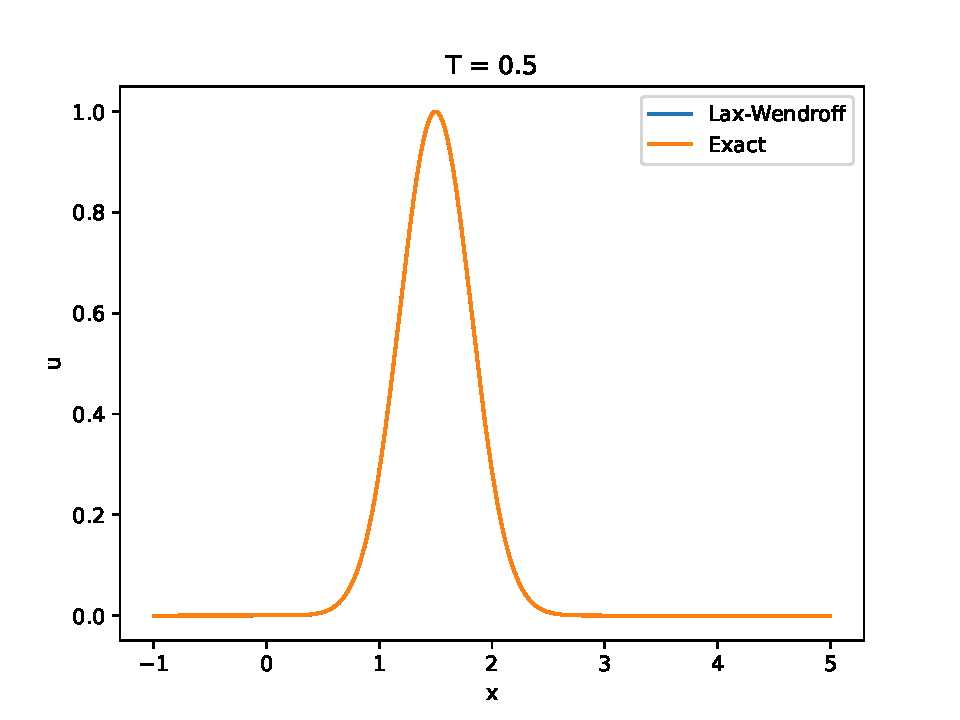
\includegraphics[scale=0.7]{3_3_LW_0_5.pdf}
		\caption{T = 0.5时使用Lax-Wendroff格式求解与精确解的对比}
		\label{3-3-LW-T0.5}
	\end{figure}

	\begin{figure}[htbp]
		\centering
		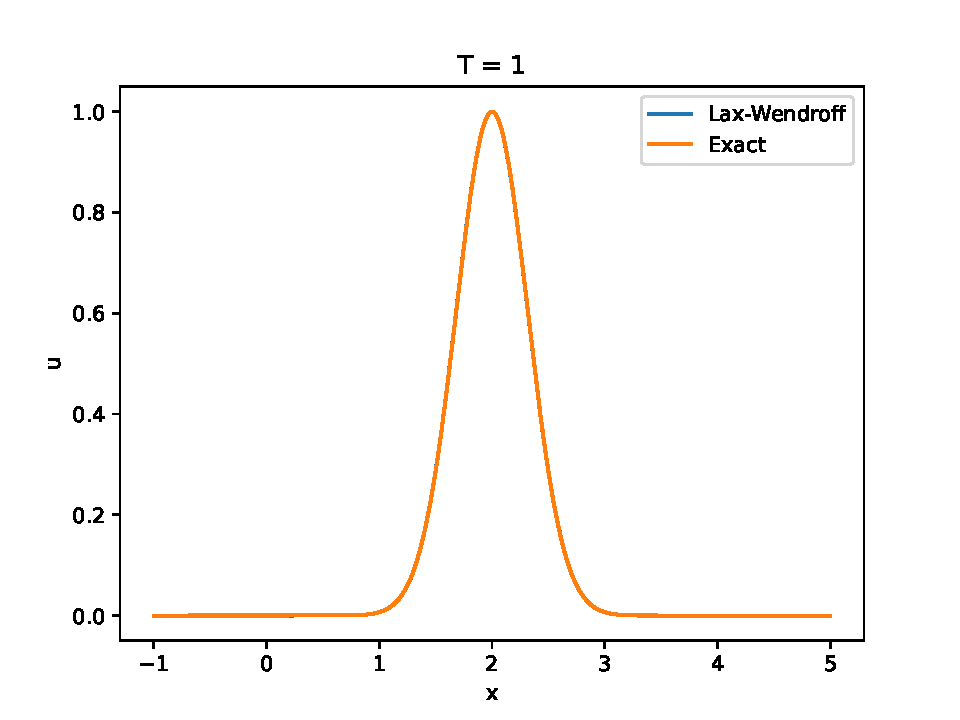
\includegraphics[scale=0.7]{3_3_LW_1_0.pdf}
		\caption{T = 1.0时使用Lax-Wendroff格式求解与精确解的对比}
		\label{3-3-LW-T1.0}
	\end{figure}

	\begin{figure}[htbp]
		\centering
		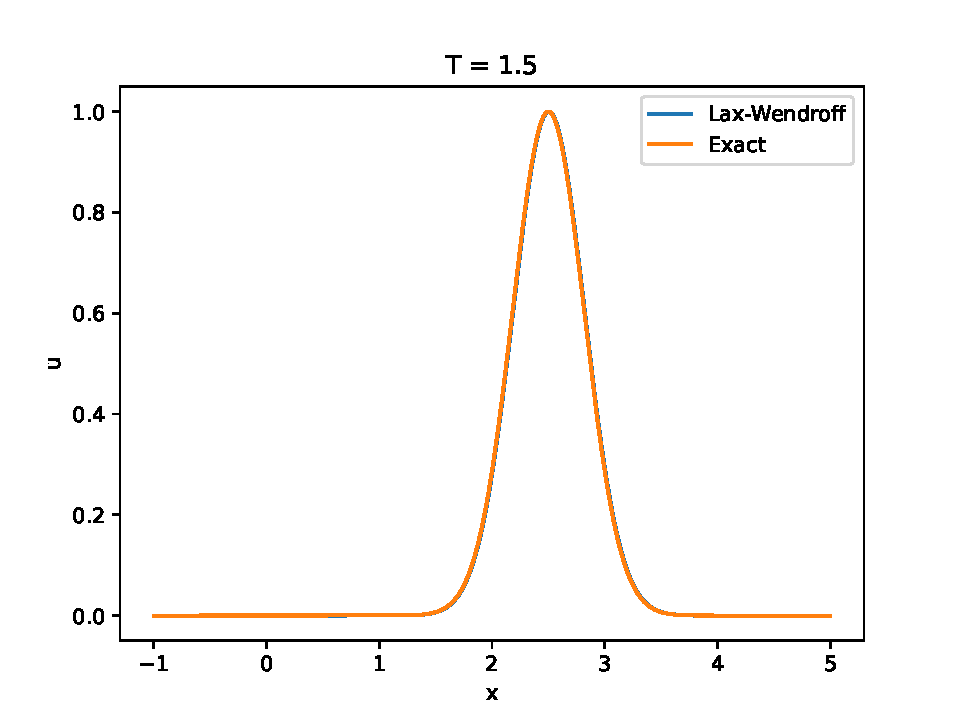
\includegraphics[scale=0.7]{3_3_LW_1_5.pdf}
		\caption{T = 1.5时使用Lax-Wendroff格式求解与精确解的对比}
		\label{3-3-LW-T1.5}
	\end{figure}

	\begin{figure}[htbp]
		\centering
		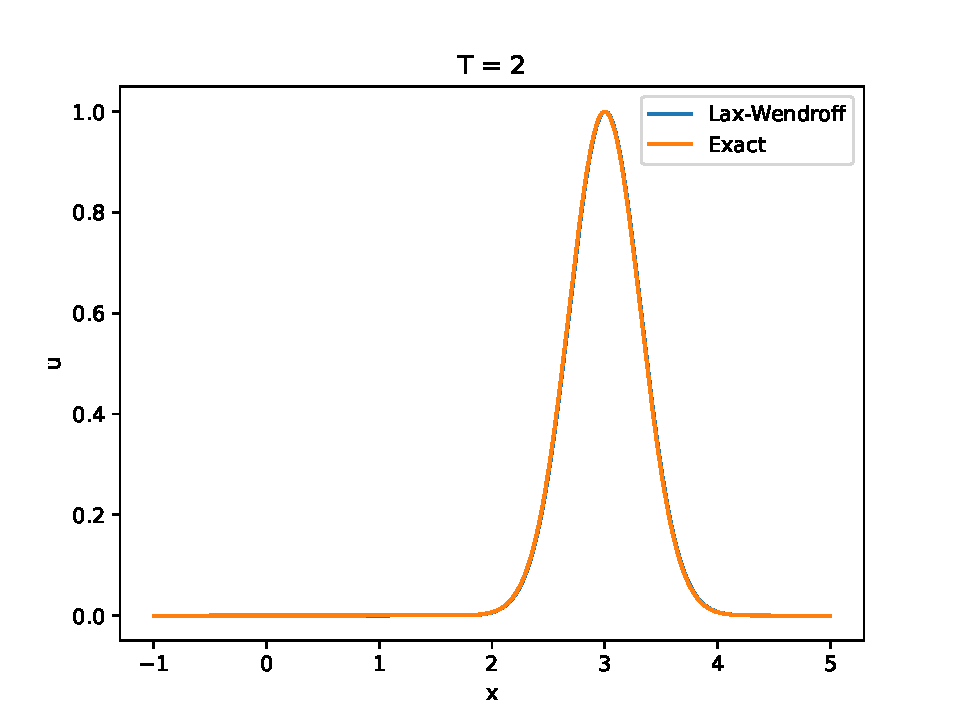
\includegraphics[scale=0.7]{3_3_LW_2_0.pdf}
		\caption{T = 2.0时使用Lax-Wendroff格式求解与精确解的对比}
		\label{3-3-LW-T2.0}
	\end{figure}
	从图中可以看出, Lax-Wendroff作为一种高阶格式, 其精度相较于upwind有着本质的提升, 仔细
	比较可以看出, 数值解在振幅和最值的角度很好地逼近了精确解, 而在相位上略慢于真实解, 这与理论上对
	Lax-Wendroff格式的增长因子的分析是一致的($O(\Delta x^3)$的振幅误差, $O(\Delta x^2)$的相对相位误差). 



\end{document}